\begingroup
\setlength{\abovedisplayskip}{6pt}
\setlength{\belowdisplayskip}{6pt}
\setlength{\abovedisplayshortskip}{4pt}
\setlength{\belowdisplayshortskip}{4pt}
\setlength{\intextsep}{6pt}

\textbf{C.2.1. Cross-sectional stiffness.} The cross section is rectangular with width \(b\) and vertical bending depth \(h\). Since the beam deflects vertically, the distance from the neutral axis is measured through \(h\), so the second moment of area is

\[
I=\frac{bh^3}{12}.
\]

Multiplying by the elastic modulus gives the cross-sectional stiffness

\[
EI=E\frac{bh^3}{12}.
\]

\[
\boxed{I=\frac{bh^3}{12},
\qquad EI=\frac{Ebh^3}{12}}
\qquad\text{(C.2.1)}
\]

\textbf{C.2.2. Spring constant.} For a concentrated tip load \(P\), the fixed-free beam tip deflection is

\[
\Delta_{\max}=\frac{PL^3}{3EI}.
\]

The equivalent tip spring constant is the load divided by the tip deflection. Therefore,

\[
k=\frac{P}{\Delta_{\max}}
 =\frac{3EI}{L^3}
 =\frac{3Ebh^3}{12L^3}.
\]

\[
\boxed{k=\frac{3EI}{L^3}}
\qquad\text{(C.2.2)}
\]

\textbf{C.2.3(a). Weight.} The gravitational force acting on the tip mass is

\[
W=mg.
\]

\[
\boxed{W=mg}
\qquad\text{(C.2.3.a)}
\]

\textbf{C.2.3(b) and C.2.4(a). Free-body diagrams.} The left panel shows the mass at static equilibrium, and the right panel shows the same mass displaced downward by \(u(t)\) from equilibrium. The cantilever is represented by its equivalent vertical spring.

\begin{figure}[H]
\centering
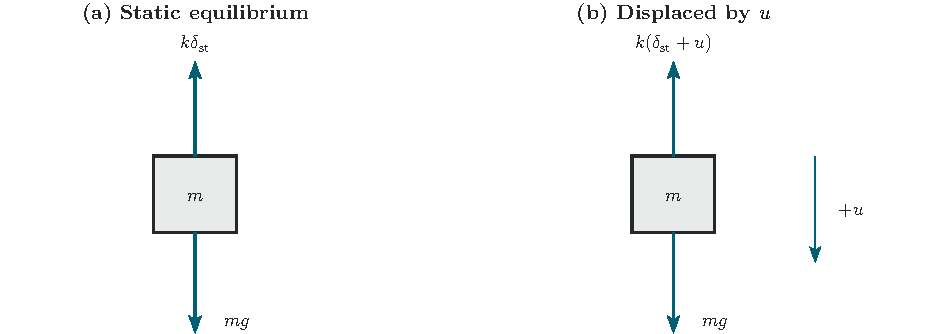
\includegraphics[width=0.95\linewidth,height=0.30\textheight,keepaspectratio,alt={Free-body diagrams for static equilibrium and vertical flex-beam vibration in Problem C.2.}]{figures/generated/solutions/vertical_fbd.pdf}
\caption{C.2.3.b and C.2.4.a. Free-body diagrams for static equilibrium and vertical flex-beam vibration.}
\end{figure}

\textbf{C.2.3(c). Static equilibrium equation.} With downward positive, the mass is stationary when the weight is balanced by the upward beam reaction. The equivalent spring force at the static deflection is \(k\delta_{\mathrm{st}}\), so

\[
\sum F_y=mg-k\delta_{\mathrm{st}}=0.
\]

\[
\boxed{mg-k\delta_{\mathrm{st}}=0}
\qquad\text{(C.2.3.c)}
\]

\textbf{C.2.3(d). Static displacement.} Solving the equilibrium equation for the deflection gives

\[
\delta_{\mathrm{st}}=\frac{mg}{k}
 =\frac{mgL^3}{3EI}.
\]

\[
\boxed{\delta_{\mathrm{st}}=\frac{mg}{k}
 =\frac{mgL^3}{3EI}}
\qquad\text{(C.2.3.d)}
\]

\textbf{C.2.4(b). Equation of motion.} Since the vibration displacement is measured from static equilibrium, the absolute downward position is

\[
y(t)=\delta_{\mathrm{st}}+u(t).
\]

The beam deformation is then \(\delta_{\mathrm{st}}+u(t)\), which gives the net vertical force

\[
\sum F_y=mg-k\bigl(\delta_{\mathrm{st}}+u(t)\bigr)
 =\bigl(mg-k\delta_{\mathrm{st}}\bigr)-ku(t).
\]

The first parenthesis vanishes by static equilibrium. Since \(\delta_{\mathrm{st}}\) is constant, \(\ddot y=\ddot u\), and Newton's law gives

\[
m\ddot{u}(t)=\sum F_y=-ku(t).
\]

Therefore, the vertical flex-beam equation of motion is

\[
\boxed{m\ddot{u}(t)+ku(t)=0}
\qquad\text{(C.2.4.b)}
\]

\textbf{C.2.4(c). Comparison with C.4.} The horizontal flex-beam model used in C.4 has the same lumped-mass equation because its cantilever is also replaced by the equivalent tip stiffness \(k=3EI/L^3\). After the displacement is measured from equilibrium, both systems reduce to

\[
\ddot{u}(t)+\frac{k}{m}u(t)=0,
\qquad
\omega_n=\sqrt{\frac{k}{m}}
 =\sqrt{\frac{3EI}{mL^3}}.
\]

The orientation affects which cross-sectional dimension is cubed in \(I\), while gravity affects the vertical system's static offset. Neither changes the form of the incremental free-vibration equation.

\[
\boxed{m\ddot{u}(t)+ku(t)=0,
\qquad \omega_n=\sqrt{\frac{3EI}{mL^3}}}
\qquad\text{(C.2.4.c)}
\]

\textbf{C.2.5. Arbitrary force field.} Let \(F(y,t)\) be the force magnitude and let \(\theta(y,t)\) be its angle from the downward vertical. Its component along the beam's allowed motion is

\[
Q(y,t)=F(y,t)\cos\theta(y,t).
\]

The absolute vertical equation becomes

\[
m\ddot{y}+ky=mg+Q(y,t).
\]

For a time-independent field, let \(y_e\) satisfy \(ky_e=mg+Q(y_e)\). Setting \(y=y_e+u\) and subtracting the equilibrium equation gives

\[
m\ddot{u}+ku=Q(y_e+u)-Q(y_e).
\]

If the field is differentiable and the vibration is small, then

\[
Q(y_e+u)-Q(y_e)\approx Q'(y_e)u,
\]

so the linearized equation is

\[
\boxed{m\ddot{u}+\bigl[k-Q'(y_e)\bigr]u=0}
\qquad\text{(C.2.5)}
\]

A constant force component only shifts the equilibrium. A position-dependent component changes the effective stiffness, and a time-dependent component remains as an external forcing term. A perpendicular component is carried by the support only in the one-coordinate model; otherwise, the model must include additional coupled motion.

\endgroup
